\section{ تبدیل فوریه دو بعدی}

الف) در ابتدا بررسی کنید برای توابع دومتغیره جدایی پذیر
$(f(x,y)=f(x)g(y))$ میتوان گفت که تبدیل فوریه آن ها
جدایی پذیر و برابر با $F(u,v)=F(u)G(v)$ است؟

\begin{qsolve}[]
	\begin{eqnarray*}
		F(u,v)&=&\intinf\intinf f(x,y)e^{-j2\pi(ux+vy)}dxdy
		=\intinf\intinf f(x)g(y)e^{-j2\pi(ux+vy)}dxdy\\
		&=&\underbrace{\left(\intinf f(x)e^{-j2\pi ux}dx\right)}_{F(u)}
		\underbrace{\left(\intinf g(y)e^{-j2\pi vy}dy\right)}_{G(v)}
		=F(u)G(v)
	\end{eqnarray*}
\end{qsolve}

ب) تبدیل فوریه و تبدیل فوریه معکوس سیگنال های زیر را محاسبه کنید. و در هر مورد شکل متناسب با پارامتر های مسئله
را رسم کنید.

\begin{qsolve}[محاسبه تبدیل فوریه یا معکوس]
	\begin{latin}
		\textbullet $f(x,y)=\frac{1}{2}\left(\delta(x-b,y-a)+\delta(x+b,y+a)\right)$
	\end{latin}
	\begin{qsolve}[]
		\begin{eqnarray*}
			F(u,v)&=&\intinf\!\intinf f(x,y)e^{-j2\pi(ux+vy)}dxdy\\
			&=&\intinf\!\intinf\frac{1}{2}\delta(x-b,y-a)e^{-j2\pi(ux+vy)}dxdy\\
			\dots&+&\intinf\!\intinf\frac{1}{2}\delta(x+b,y+a)e^{-j2\pi(ux+vy)}dxdy\\
			&=&\frac{1}{2}e^{-j2\pi(ux+vy)}\when_{x=b,y=a}+\frac{1}{2}e^{-j2\pi(ux+vy)}\when_{x=-b,y=-a}\\
			&=&
			\frac{1}{2}\left(e^{j2\pi(ub+va)}+e^{-j2\pi(ub+va)}\right)\\
			&=&\cos(2\pi(ub+va))=F(u,v)\Longrightarrow\qquad\text{\hl{$F(u,v)=\cos(2\pi(ub+va))$}}
		\end{eqnarray*}
		\begin{center}
			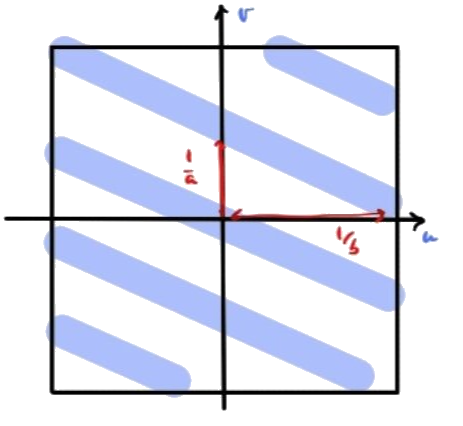
\includegraphics[width=4cm]{pics/q4_2_1.png}
		\end{center}
	\end{qsolve}


	\begin{latin}
		\textbullet $f(x,y)=\begin{cases}
				e^{-|x|-|y|} & -1\leq x\leq 1 \text{and} -1\leq y\leq 1 \\
				0            & \text{otherwise}
			\end{cases}$
	\end{latin}

	\splitqsolve
	\begin{qsolve}[]
		\begin{eqnarray*}
			F(u,v)&=&\intinf\!\intinf f(x,y)e^{-j2\pi(ux+vy)}dxdy=
			\int_{-1}^{1}\!\int_{-1}^{1} e^{-|x|-|y|}e^{-j2\pi(ux+vy)}dxdy\\
			&=&\underbrace{\left(\int_{-1}^{1}e^{-|x|-j2\pi ux}dx\right)}_{g(u)}
			\underbrace{\left(\int_{-1}^{1}e^{-|y|-j2\pi vy}dy\right)}_{g(v)}=g(y)g(v)\\
			% \end{eqnarray*}
			% \begin{eqnarray*}
			g(m)&=&\int_{-1}^{1}e^{-|t|-j2\pi mt}dt=\int_{0}^{1}e^{-t-j2\pi mt}dt+\int_{-1}^{0}e^{t-j2\pi mt}dt\\
			&=&\frac{1}{1+j2\pi m}\left(1-e^{-1-j2\pi m}\right)+\frac{1}{1-j2\pi m}\left(1-e^{-1+j2\pi m}\right)\\
			&=&
			\frac{2}{1+4\pi^2m^2}-e^{-1}\frac{(1-j2\pi m)e^{-j2\pi m}+(1+j2\pi m)e^{j2\pi m}}{1+4\pi^2m^2}\\
			g(m)&=&\frac{2\left(
				1-e^{-1}\cos(2\pi m)+e^{-1}2\pi m\sin(2\pi m)
				\right)}{1+4\pi^2m^2}\Rightarrow\\
			F(u,v)&=&\frac{4\left[1-e^{-1}(\cos(2\pi v)-2\pi v\sin(2\pi v))\right]
			\left[1-e^{-1}(\cos(2\pi u)-2\pi u\sin(2\pi u))\right]}
			{(1+4\pi^2v^2)(1+4\pi^2u^2)}
		\end{eqnarray*}
		\centerline{\hl{$
			F(u,v)=\frac{4\left[1-e^{-1}(\cos(2\pi v)-2\pi v\sin(2\pi v))\right]
			\left[1-e^{-1}(\cos(2\pi u)-2\pi u\sin(2\pi u))\right]}
			{(1+4\pi^2v^2)(1+4\pi^2u^2)}$}}

		شمای دقیق کشیدن بسیار دشوار بوده، در فواصل دور به تقریب شبیه 2 تا sinc میباشد.

		\begin{center}
			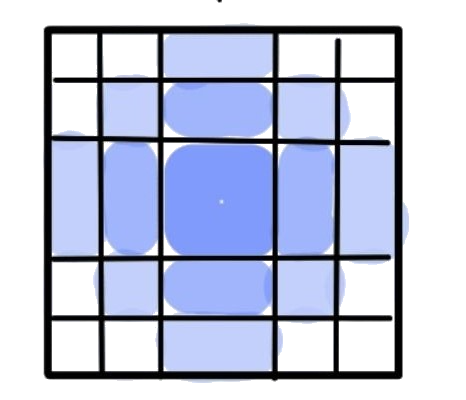
\includegraphics[width=4cm]{pics/q4_2_2.png}
		\end{center}
	\end{qsolve}

	\begin{latin}
		\textbullet $F(u,v)=ab\cos(2\pi cv)\sinc(\pi av)\sinc(\pi bu)$
	\end{latin}

	\begin{qsolve}[]
		\begin{eqnarray*}
			G(u,v)&=&ab\sinc(\pi av)\sinc(\pi bu)\qquad F(u,v)=G(u,v)\times\cos(2\pi cv)\\
			F(u,v)&=&\frac{1}{2}e^{j2\pi cv}G(u,v)+\frac{1}{2}e^{-j2\pi cv}G(u,v),\quad g(x,y)\leftrightarrow G(u,v)\Rightarrow\\
			f(x,y)&=&\frac{1}{2}g(x,y+c)+\frac{1}{2}g(x,y-c)\\
			G(u,v)&=&\underbrace{\left(a\ \sinc(\pi av)\right)}_{H(a,v)}\underbrace{\left(b\ \sinc(\pi bu)\right)}_{H(b,u)}
			\xrightarrow{\text{قسمت الف}}g(x,y)=h(a,u)\times h(b,x)\\
			H(a,v) &=&a\ \sinc(\pi a v)\Rightarrow h(a,y)=\sqcap_a(y)\Rightarrow
			g(x,y) = \sqcap_a(y)\sqcap_b(x)\\
			f(x,y)&=&\text{\hl{$\frac{1}{2}\left(\sqcap_a(y-c)+\sqcap_a(y+c)\right)\sqcap_b(x)=f(x,y)$}},\quad \sqcap_{x_0}(x)=\begin{cases}
				1 & |x| \leq \frac{1}{2}x_0 \\
				0 & \text{otherwise}
			\end{cases}
		\end{eqnarray*}
        \splitqsolve[\splitqsolve]
        مقدار در نواحی رنگی $\frac{1}{2}$ و در باقی نواحی صفر است.
        \begin{center}
			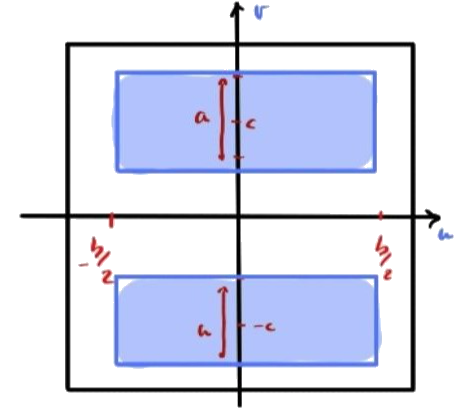
\includegraphics[width=4cm]{pics/q4_2_3.png}
		\end{center}
	\end{qsolve}

	\begin{latin}
		\textbullet $F(u,v)=\cos(2\pi av)\cos(2\pi bu)$
	\end{latin}
	\begin{qsolve}[]
		\begin{eqnarray*}
			F(u,v)&=&\underbrace{\cos(2\pi av)}_{G(a,v)}\underbrace{\cos(2\pi bu)}_{G(b,u)}
			\xrightarrow{\text{قسمت الف}}f(x,y)=g(a,y)g(b,x)\\
			G(a,v)&=&\cos(2\pi av)=\frac{1}{2}\left(e^{j2\pi av}+e^{-j2\pi av}\right)
			\Rightarrow g(a,y)=\frac{1}{2}\left(\delta(y-a)+\delta(y+a)\right)\\
			f(x,y)&=&g(a,y)g(b,x)=\frac{1}{4}\left(\delta(y-a)+\delta(y+a)\right)\left(\delta(x-b)+\delta(x+b)\right)\\
			&=&\frac{1}{4}\left(\delta(x-b,y-a)+\delta(x-b,y+a)+\delta(x+b,y-a)+\delta(x+b,y+a)\right)\\
			&=&\frac{1}{4}\delta\left(|x|-|b|,|y|-|a|\right)\qquad\text{ساده سازی برای نمایش، مرحله قبل توصیفی تر بوده}
		\end{eqnarray*}
		\centerline{\hl{$f(x,y)=\frac{1}{4}\delta\left(|x|-|b|,|y|-|a|\right)$}}
        \begin{center}
			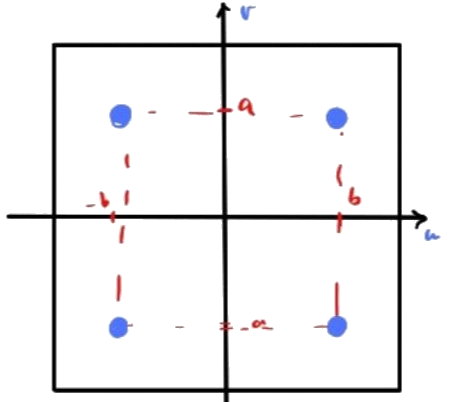
\includegraphics[width=4cm]{pics/q4_2_4.png}
		\end{center}
	\end{qsolve}
\end{qsolve}